\documentclass{beamer}
% theme général du diaporama
\usetheme{Boadilla}
%paquets pour le français
\usepackage[T1]{fontenc}
\usepackage[utf8]{inputenc}
\usepackage{hyperref}

%package pour les images
\usepackage{graphicx}

\subtitle{}
\title{Compression d'image via la méthode Run-Length-Encoding}
\institute[Paris 8]{Paris VIII}
\author{Chaolei CAI}
\date{\today}
%modifie le fond de la presentation
\setbeamercolor{background canvas}{bg = white}
%\setbeamercovered{transparent}
%\usecolortheme[named=gray]{structure}


\begin{document}

    \frame{\titlepage}
    \tableofcontents

    \section{Presentation de l'algorithme}

    \begin{frame}
        \frametitle{Qu'est qu'une image?}
        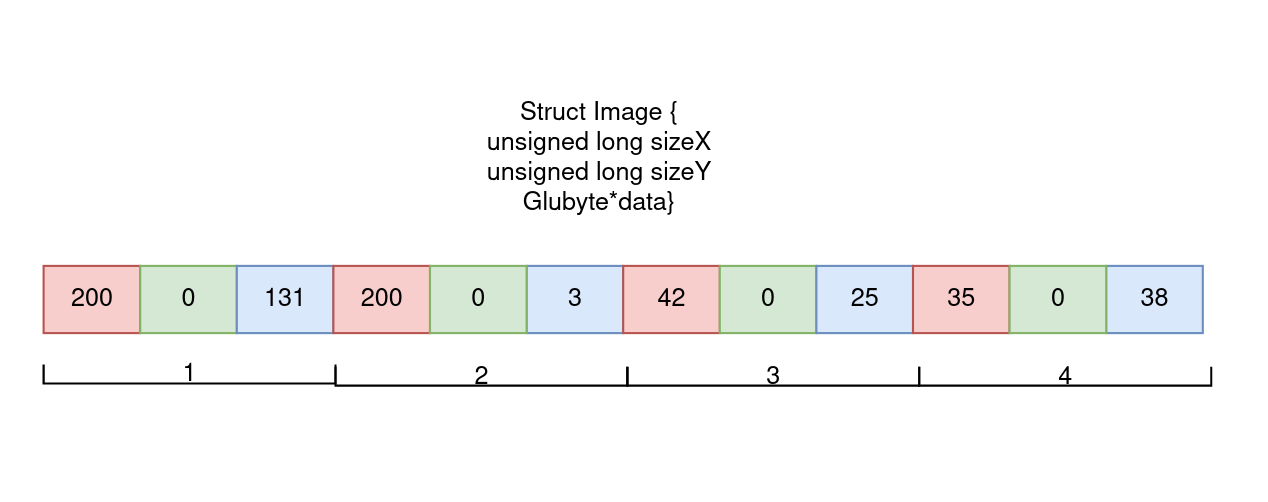
\includegraphics[width=\linewidth]{img/fig1.png}
    \end{frame}    
    
    \begin{frame}
        \frametitle{Compression?}
        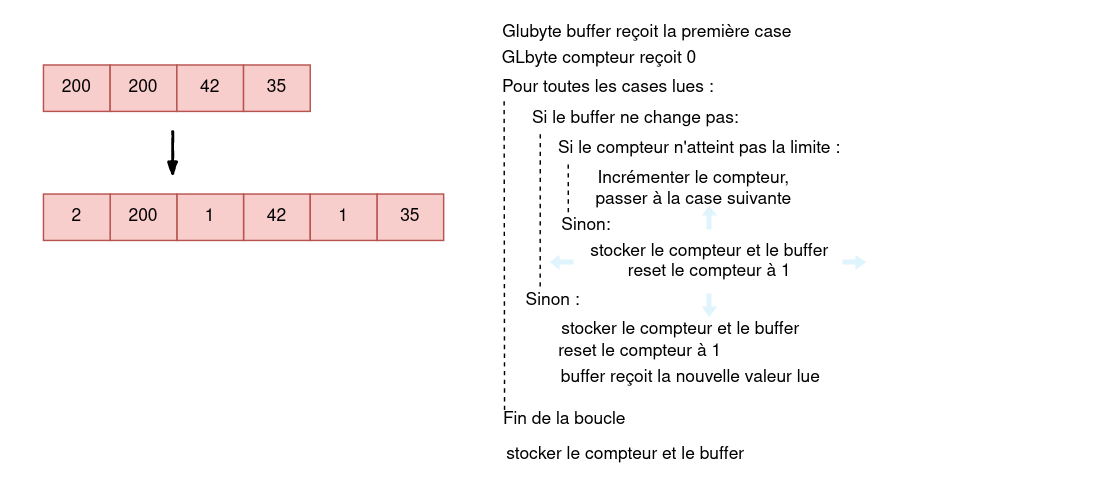
\includegraphics[width=\linewidth]{img/fig2.png}
    \end{frame}
    
    \begin{frame}
        \frametitle{Cas idéal}
        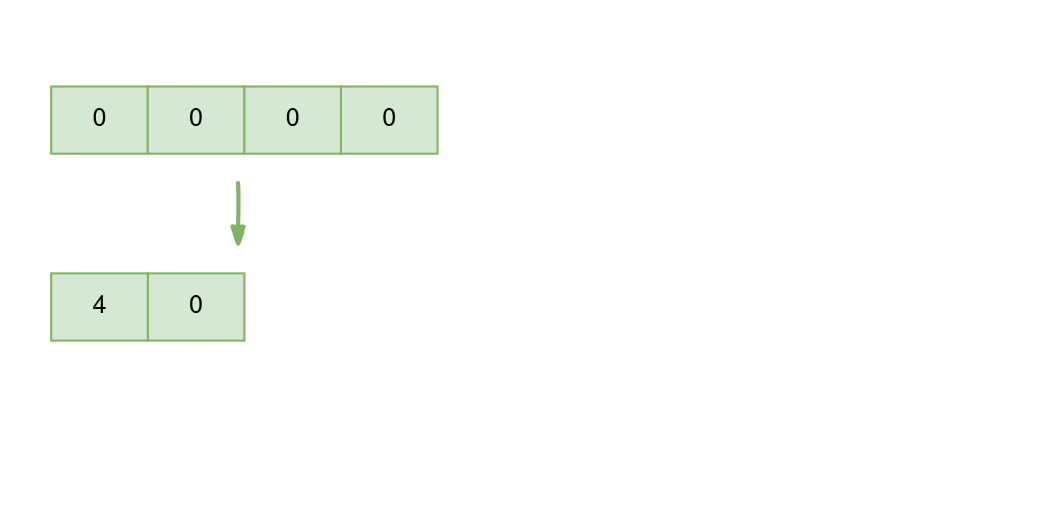
\includegraphics[width=\linewidth]{img/fig3.png}
    \end{frame}

    \begin{frame}
        \frametitle{Pire cas possible}
        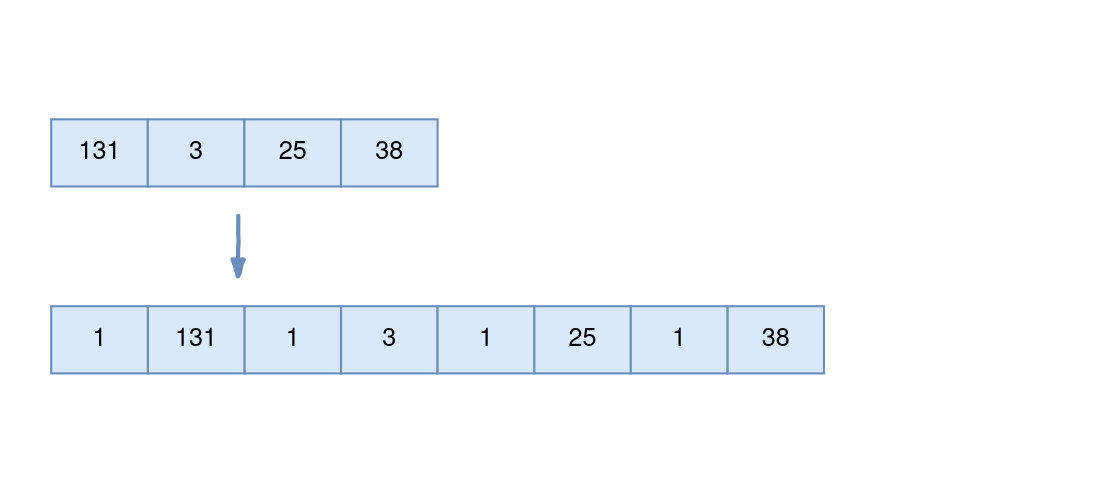
\includegraphics[width=\linewidth]{img/fig4.png}
    \end{frame}

    \section{Version améliorée de l'algorithme}
    \begin{frame}
        \frametitle{Méthode améliorée par Silicon Graphics International}
        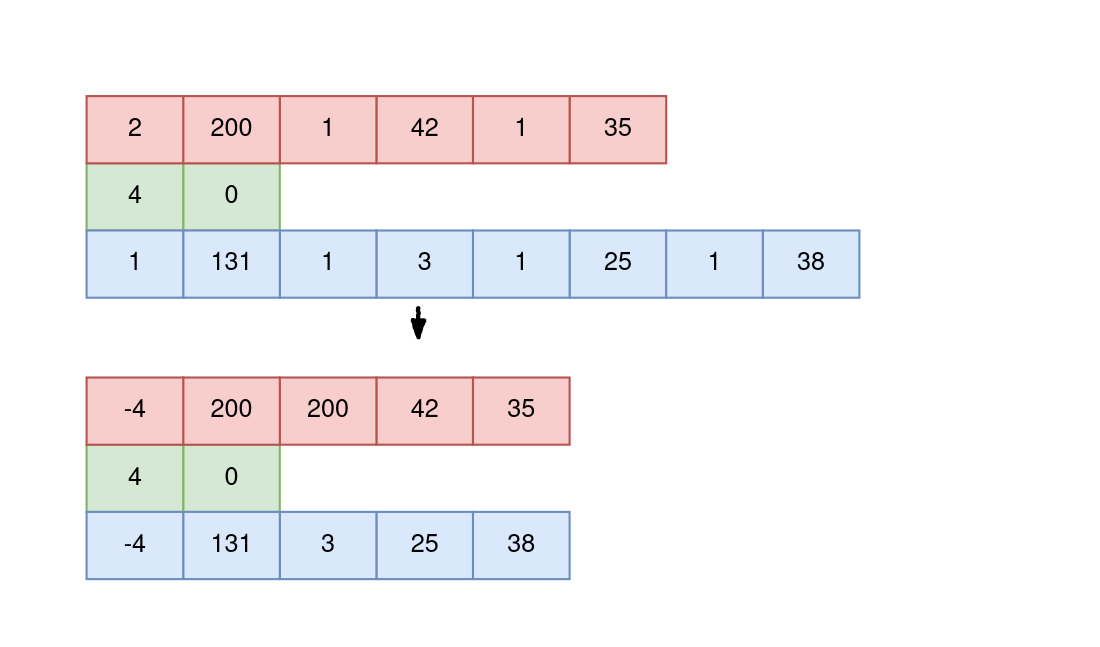
\includegraphics[width=\linewidth]{img/fig5.png}
    \end{frame}   
    
    \begin{frame}
        \frametitle{Seconde compression à appliqué sur le résultat précedente}
        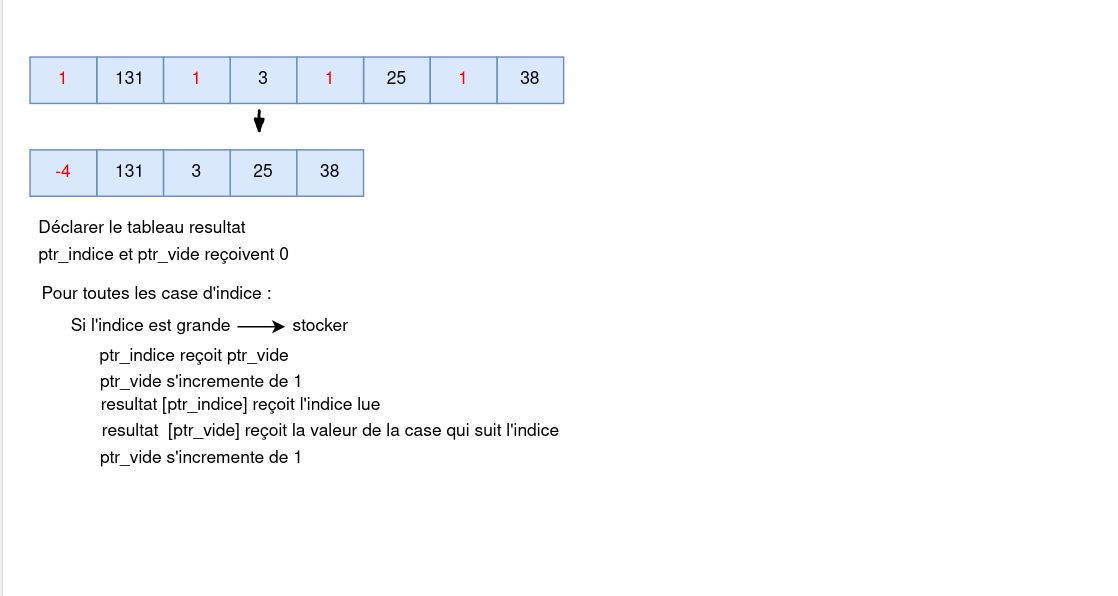
\includegraphics[width=\linewidth]{img/fig7.png}
    \end{frame}   
    
    \begin{frame}
        \frametitle{Pseudo-code de la réduction}
        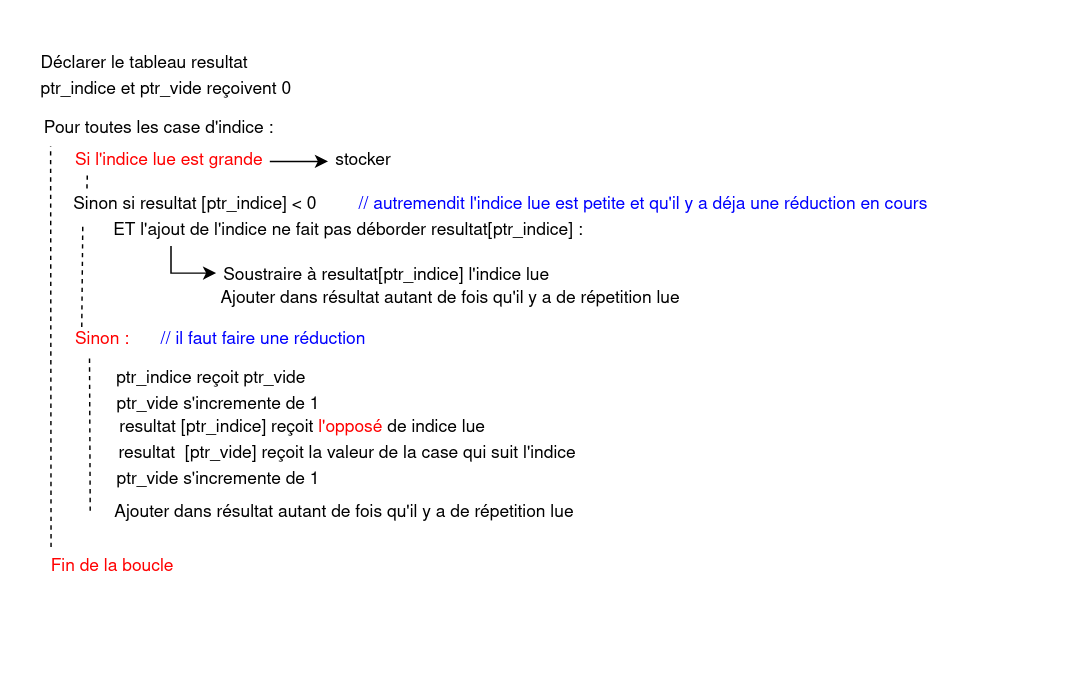
\includegraphics[width=\linewidth]{img/fig8.png}
    \end{frame}   
    
    
    \begin{frame}
        \frametitle{Nouvelle structure d'image}
        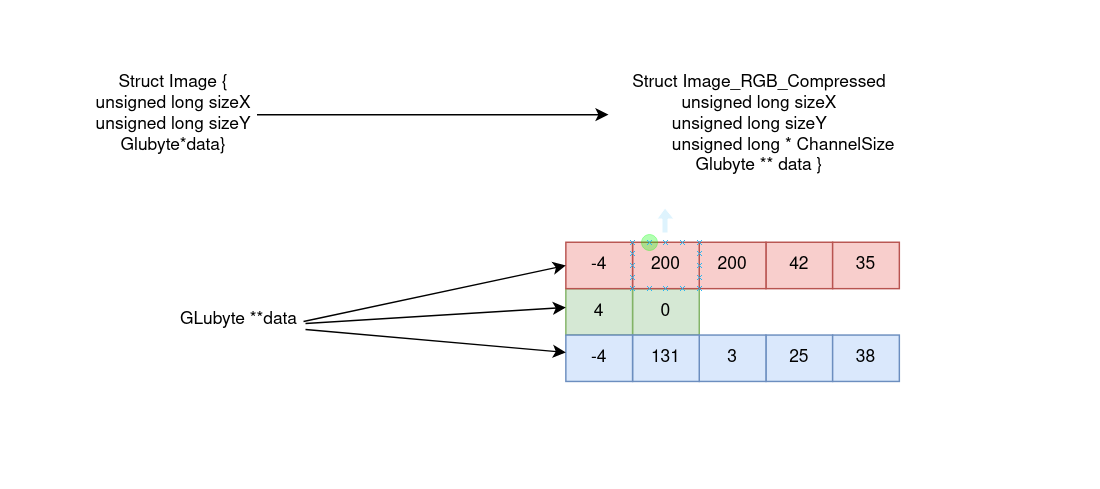
\includegraphics[width=\linewidth]{img/fig6.png}
    \end{frame}
    
    \section{Différence entre le RGB et le HSV}
    \begin{frame}
        \frametitle{Cube RGB}
        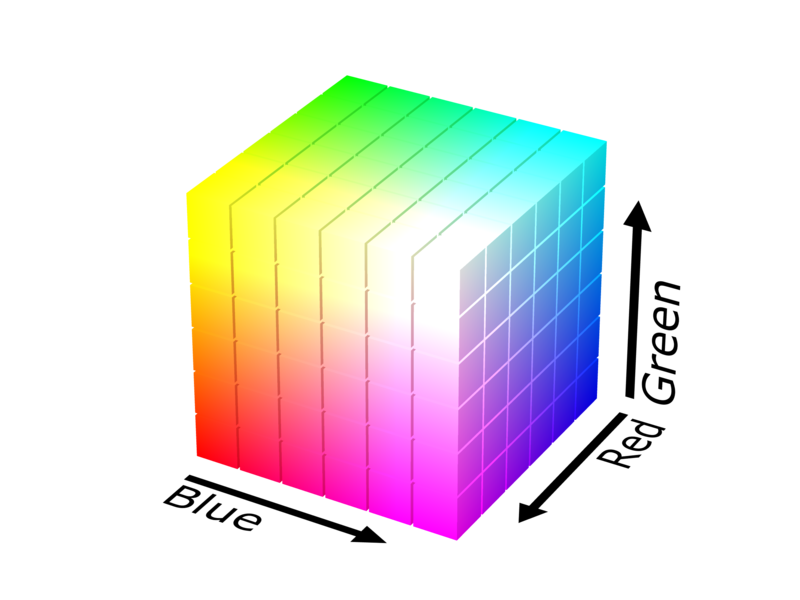
\includegraphics[width=\linewidth]{img/fig9.png}
    \end{frame}    
    
    \begin{frame}
        \frametitle{Cylindre HSV}
        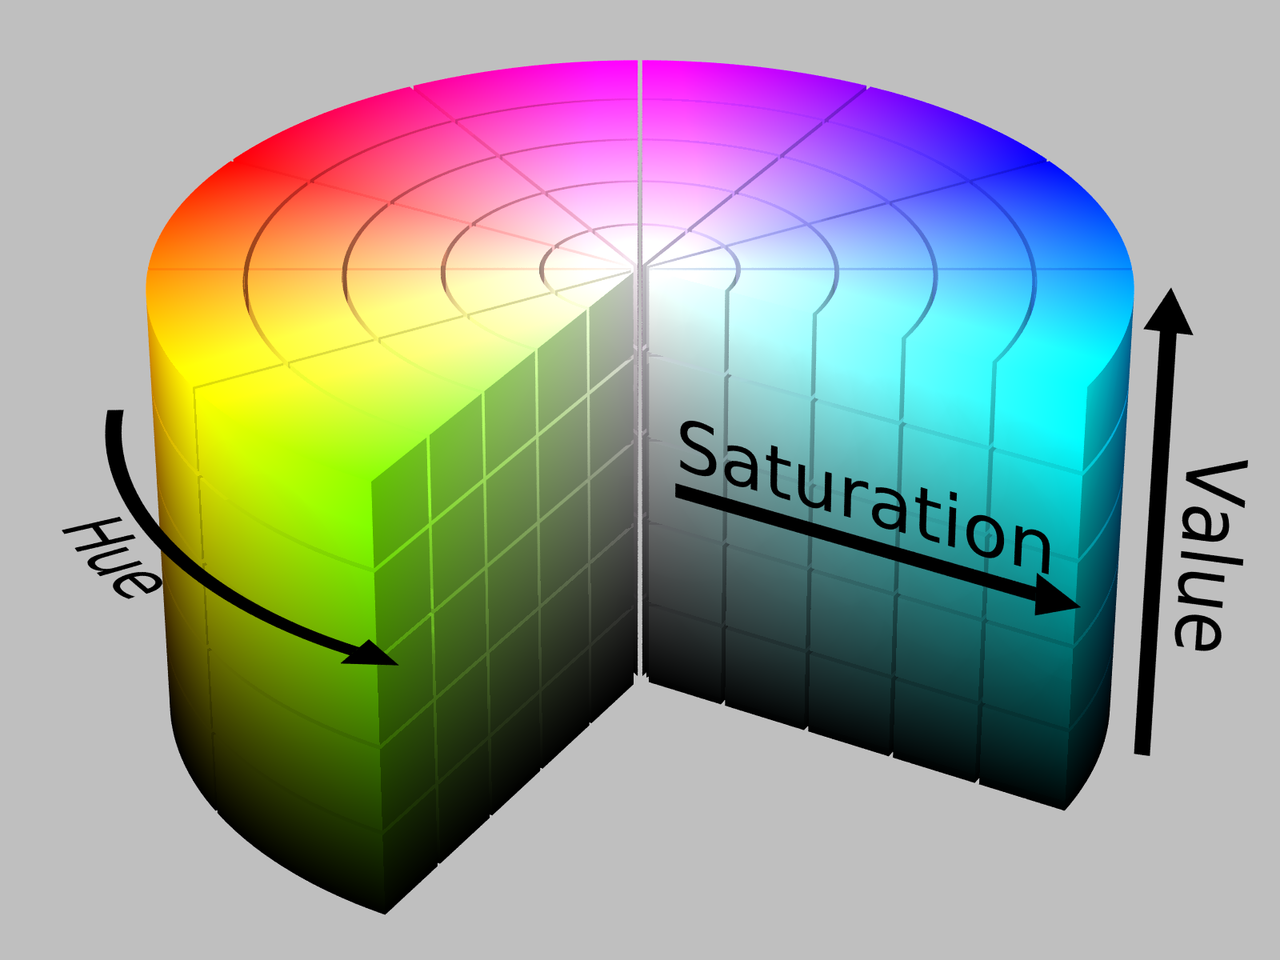
\includegraphics[width=\linewidth]{img/fig10.png}
    \end{frame}    
    
    \begin{frame}
        \frametitle{Avantages du hsv}
        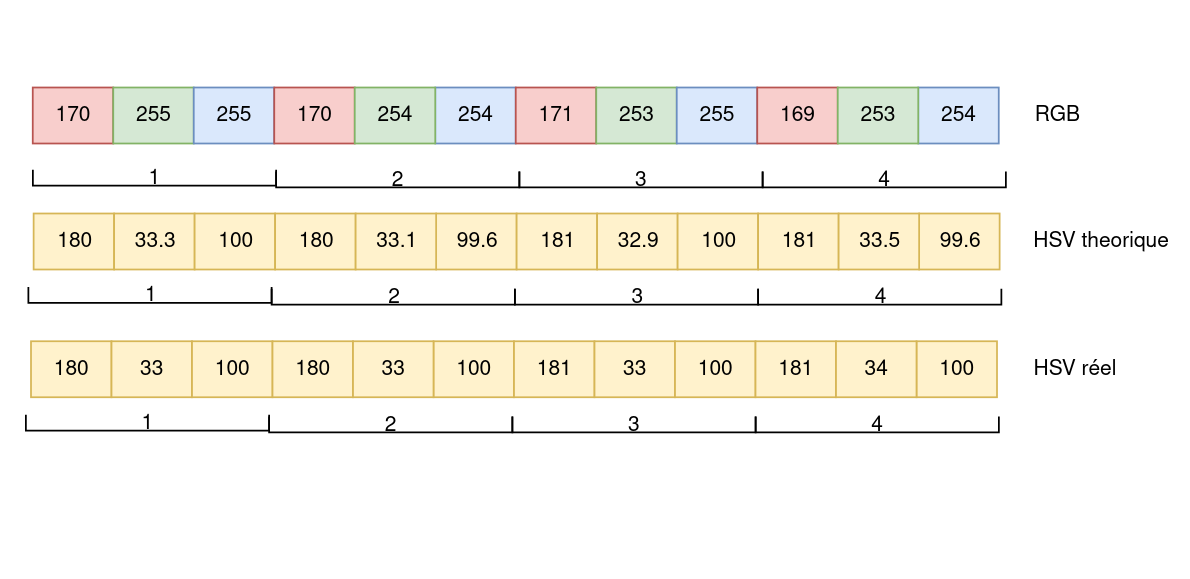
\includegraphics[width=\linewidth]{img/fig11.png}
    \end{frame}

    \section{Performances}
    \begin{frame}
        \begin{tabular}{l|l|l|l}
          Nom  & Taille initial & RGB & HSV\\
          \hline  
          can\_bottom2 & 100\% & 95.32\% & 113.76\% \\
          \hline
          chatou & 100\% & 100.17\% & 131.99\% \\
          \hline
          Cordiliere2\_V3 & 100\% & 97.72\% & 115.95\% \\
          \hline
          Kili\_mais & 100\% & 98.09\% & 125.51\%  \\
          \hline
          Refuges & 100\% & 95.32\% & 117.35\% \\
          \hline
          requin\_leopard & 100\% & 100.16\% & 131.63\% \\
          \hline
          comic & 100\% & 72.52\% & 88.15\% \\
          \hline
          mickey & 100\% & 26.11\% & 26.18\%\\
          \hline
          morty & 100\% & 49.76\% & 59.25\% \\
          \hline
          morty\_with\_imagesave & 100\% & 49.75\% & 59.25\% \\
          \hline
          green & 100\% & 1.57\% & 1.05\% \\
        \end{tabular}\\
        Moyennes élaguées:\\
        \textbf{76\%} sous RGB, et \textbf{93\%} sous HSV 
    \end{frame}

    \begin{frame}
        \frametitle{Optimisation possible}
        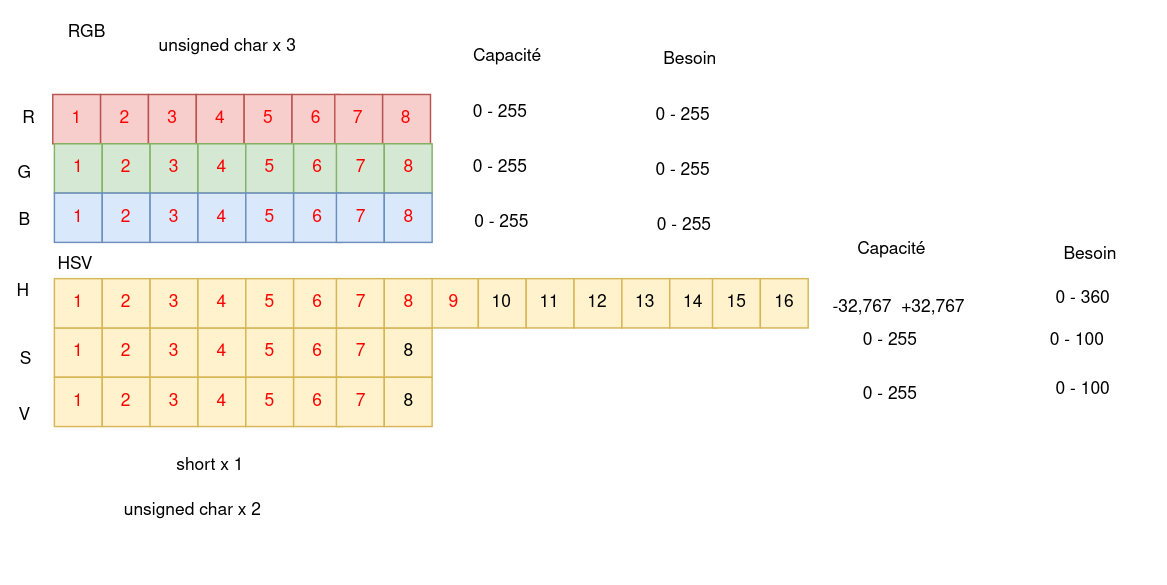
\includegraphics[width=\linewidth]{img/fig12.png}
    \end{frame}

    

    \begin{frame}
        \frametitle{Sources}
        \href{https://commons.wikimedia.org/wiki/File:RGB_color_solid_cube.png}{Cube RGB}\\
        \href{https://en.wikipedia.org/wiki/HSL_and_HSV\#/media/File:HSV_color_solid_cylinder_saturation_gray.png}{Cylindre HSV}


    \end{frame}

\end{document}
